\documentclass[
10pt,
aspectratio=169,
]{beamer}


\usepackage{lipsum}
\usepackage{tikz}

\title{TP Traitements Numériques Avancés}
\subtitle{Ecouteurs à réduction de bruit}
\date{Promo ESE 2022}
\author{Nicolas Guérin et Emma Perret}
%\institute{date}

\usetheme{ensea}  


\begin{document}

\begin{frame}
\titlepage
\end{frame}

%%% INTRODUCTION %%%
\section{Introduction}
\begin{frame} 
\frametitle{Introduction} 
Pour chaque bloc il faut réfléchir aux fréquences d'échantillonnage et de coupure mais également à la bande passante et au gain de cette bande. Il faut également penser à l'ordre du filtre. Pour chauqe signal, la fréquence d'échantillonnage et la longueur des mots sont déjà donnés.\\
Pour un signal PCM, nous pouvon facilement trouver la bande passante et le rapport signal à bruit :
\begin{enumerate} 
\item La bande passante équivaut à la fréquence d'échantillonnage ($f_e ~ ou ~ f_s$) divisée par deux.
\item Le rapport signal à bruit ($RSB ~ ou ~ SNR$) se définit de la sorte : $RSB = 6.02 * N + 1.76 $ avec $N ~ : ~ la ~ longueur ~ des ~ mots$. Il s'exprime en $dB$.
\item Pour un signal sur 16 bits, $RSB = 98 dB$.
\item Nous acceptons un $RSB - 4dB$. Pour cela, nous sommes obligés de passer par un dithering. Sans le dithering, le $RSB$ est de $-8 dB$ ce qui n'est pas acceptable.
\end{enumerate}
\end{frame}

\begin{frame} 
\frametitle{Introduction} 
Nous avons donc listé les données pour tous les signaux PCM.\\
Pour le signal de sortie de l'égalisateur : 
\begin{enumerate} 
\item $f_e = 48 kHz$
\item $Bande-passante = f_e/2 = 24 kHz$
\item $N = 20 bits$
\item $RSB = 122.16 dB$
\item $RSB ~accepté = RSB - 4 = 118.16 dB$
\end{enumerate}
\vspace*{0.7cm}
Pour le signal de sortie du SR converter : 
\begin{enumerate} 
\item $f_e = 48 kHz$
\item $Bande-passante = f_e/2 = 24 kHz$
\item $N = 16 bits$
\item $RSB = 98.08 dB$
\item $RSB ~accepté = RSB - 4 = 94.08 dB$
\end{enumerate}
\end{frame}

\begin{frame} 
\frametitle{Introduction} 
Pour le signal de sortie du player audio : 
\begin{enumerate} 
\item $f_e = 44.1 kHz$
\item $Bande-passante = f_e/2 = 22.05 kHz$
\item $N = 16 bits$
\item $RSB = 98.08 dB$
\item $RSB ~accepté = RSB - 4 = 94.08 dB$
\end{enumerate}
\vspace*{0.7cm}
Pour les signaux de sortie du micro et du PDM modulator : 
\begin{enumerate} 
\item $f_e = 6.144 MHz$
\item $Bande-passante = f_e/2 = 3.72 MHz$
\item $N = 1 bits$
\item $RSB = 122.16 dB$
\item $RSB~accepté = RSB - 4 = 118.16 dB$
\end{enumerate}
\end{frame}
%%% FIN INTRODUCTION %%%

%%% PARTIE 1 : PDM %%%
\section{Partie 1 : PDM}
\begin{frame} 
\frametitle{Partie 1 : PDM demodulator - PDM modulator} 
\framesubtitle{Modulateur PDM} 
Le modulateur PDM permet de moduler un signal analogique en un signal binaire en fonction de la densité du signal. En effet, plus l'amplitude du signal analogique est élevée, plus le signal binaire sera constitué d'une suite longue de 1.\\
\vspace*{0.3cm}
La génération du modulteur PDM a déjà été faite. Après avoir compris son fonctionnement, nous sommes donc directement passés au démodulateur PDM.
\end{frame}

\begin{frame} 
\frametitle{Partie 1 : PDM demodulator - PDM modulator} 
\framesubtitle{Démodulateur PDM - Théorie} 
La fréquence d'échantillonnage d'entrée vaut $f_e~=~6.144~MHz$ et celle de la sortie vaut $f_e~=~48~kHz$. Il y a un rapport de 128 entre les deux.\\
Il faut sous-échantillonner mais si nous échantillonnons par 128, cela est trop brutal et entraîne un ordre de filtre trop élevé et une pulsation de coupure très faible. Il faut donc faire par étape. \\
Mais avant de sous-échantilloner il faut filtrer. Nous avons choisi de prendre un filtre FIR, cela nous permet aussi de conserver la forme du signal puisque c'est un filtre à phase linéaire. Cependant le FIR entraîne des problèmes de latence car nous avons un RSB élevé ($120 dB$). Il faut donc faire attention au délai.
\end{frame}

\begin{frame} 
\frametitle{Partie 1 : PDM demodulator - PDM modulator} 
\framesubtitle{Démodulateur PDM - Mise en place} 
Dans un premier temps nous décidons de sous-échantilloneur par 16 puis par 8 (le produit des deux donne bien 128). \\
Nous utilisons Filter Designer pour designer nos filtres FIR.\\
Pour le filtre avant le sous-échantillonneur par 16, nous prenons : 
\begin{enumerate}
    \item $f_s~=~6.144~MHz$
    \item $f_{stop}~=~f_e/16~=~384~kHz$
    \item $A_{stop}~=~120~dB$
\end{enumerate}
\vspace*{0.7cm}
Pour le filtre avant le sous-échantillonneur par 8, nous prenons : 
\begin{enumerate}
    \item $f_s~=~384~kHz$
    \item $f_{stop}~=~f_e/16~=~24~kHz$
    \item $A_{stop}~=~120~dB$
\end{enumerate}
\end{frame}

\begin{frame}
\frametitle{Partie 1 : PDM demodulator - PDM modulator} 
\framesubtitle{Démodulateur PDM - Signal d'entrée} 
Nous observons d'abord le signal d'entrée~\ref{fig:entrée} : 
\begin{figure}[h]
    \centering
    \includegraphics[scale=0.2]{Images/entrée.png}
    \caption{Signal d'entrée}
    \label{fig:entrée}
\end{figure}
\end{frame}

\begin{frame}
\frametitle{Partie 1 : PDM demodulator - PDM modulator} 
\framesubtitle{Démodulateur PDM - Filtres} 
Nous créons nos deux filtres : 
\begin{figure}[h]
    \centering
    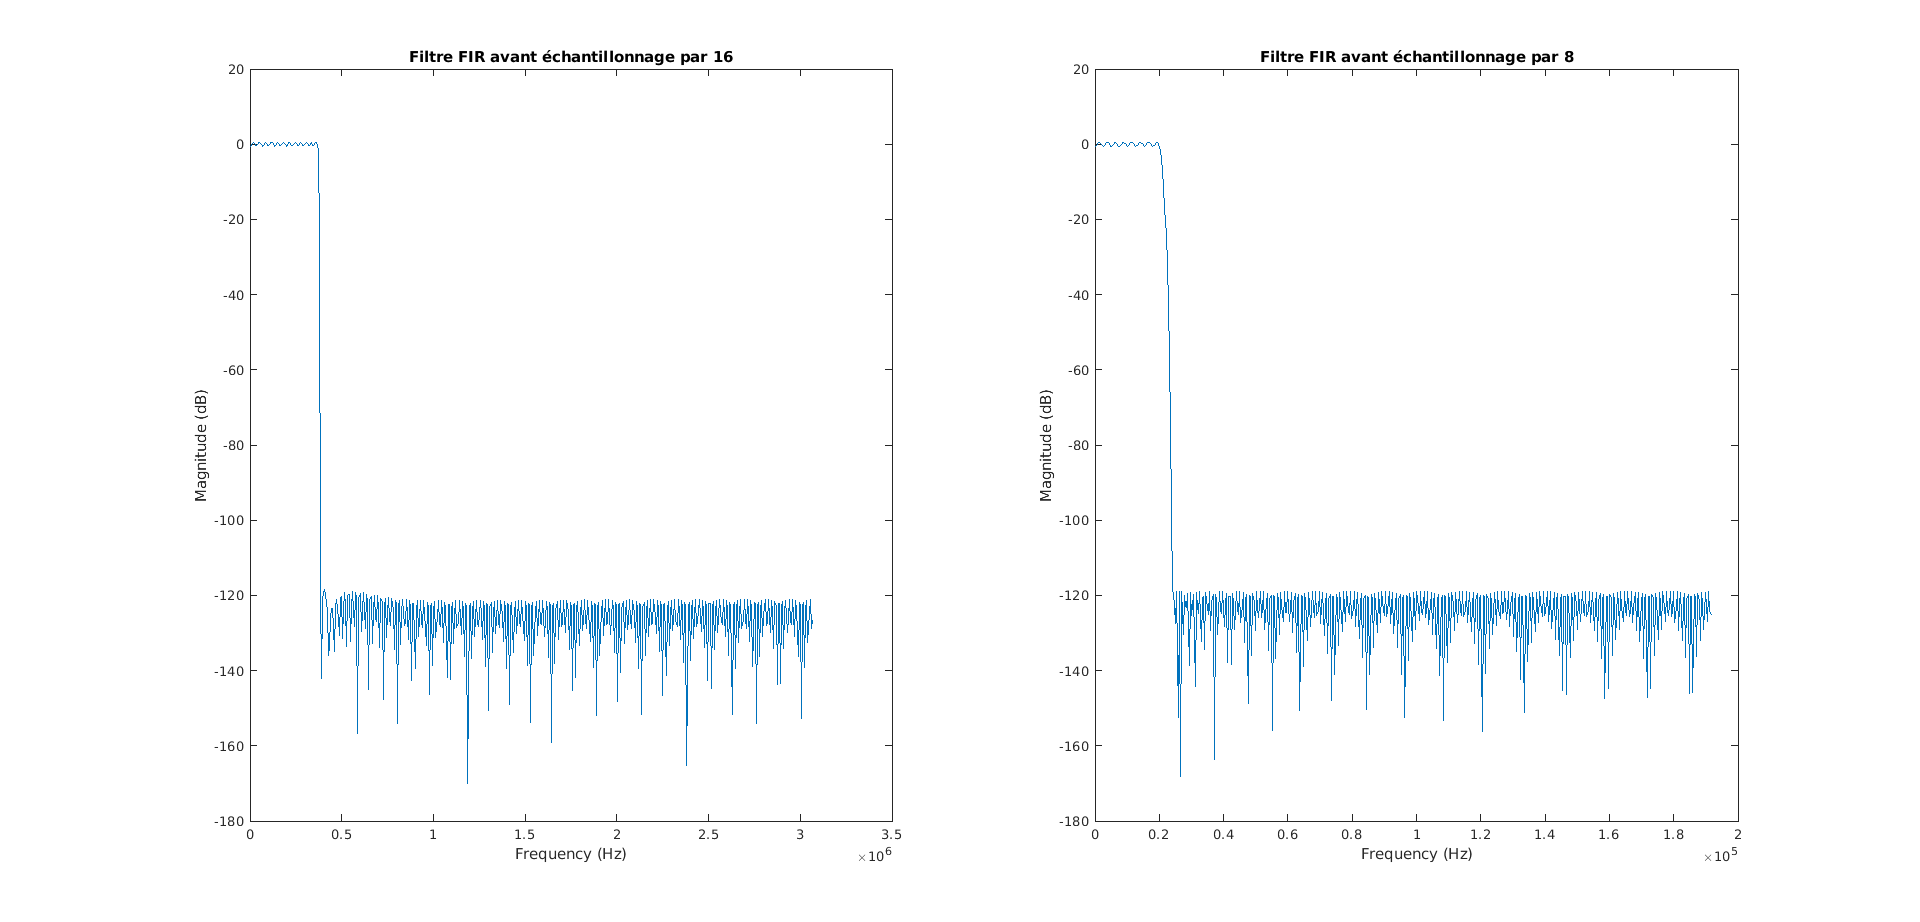
\includegraphics[scale=0.2]{Images/FIR.png}
    \caption{Filtres FIR}
    \label{fig:FIR}
\end{figure}
\end{frame}

\begin{frame}
\frametitle{Partie 1 : PDM demodulator - PDM modulator} 
\framesubtitle{Démodulateur PDM - Sortie du sous-échantillonneur par 16} 
Nous observons les sorties de chaque sous-échantillonneur : 
\begin{figure}[h]
    \centering
    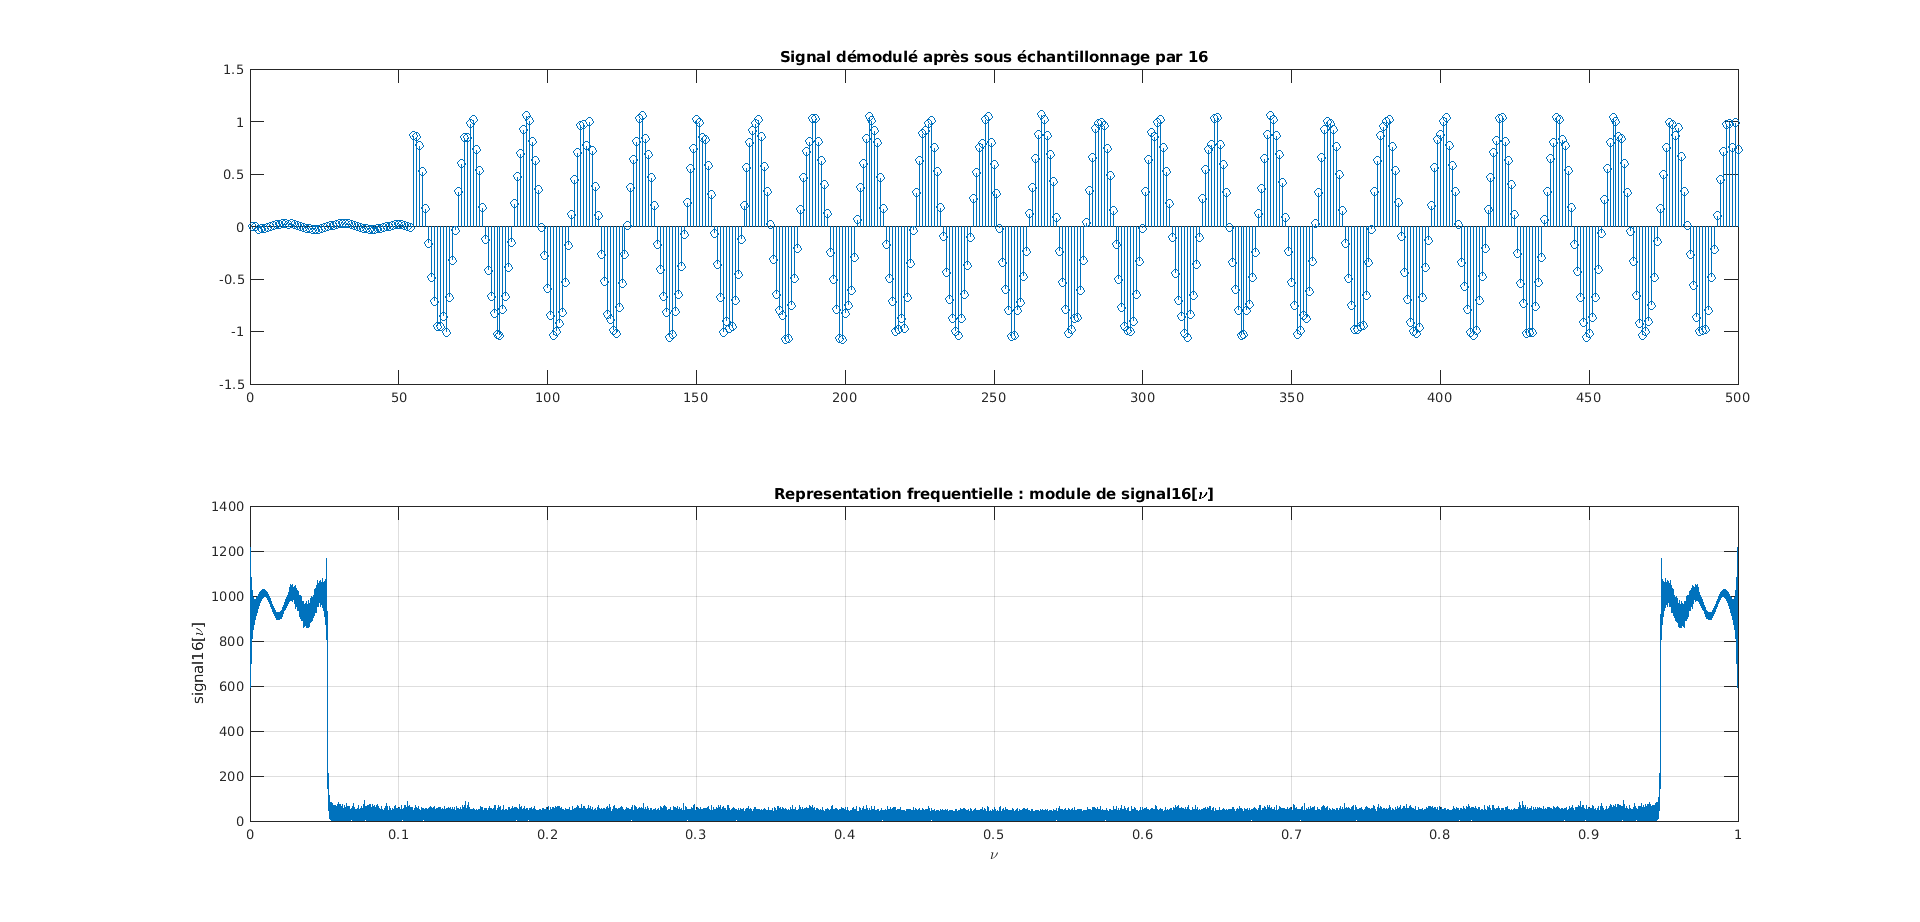
\includegraphics[scale=0.2]{Images/signal16.png}
    \caption{Sortie du sous-échantillonneur par 16}
    \label{fig:sig16}
\end{figure}
\end{frame}

\begin{frame}
\frametitle{Partie 1 : PDM demodulator - PDM modulator} 
\framesubtitle{Démodulateur PDM - Sortie du sous-échantillonneur par 8} 
\begin{figure}[h]
    \centering
    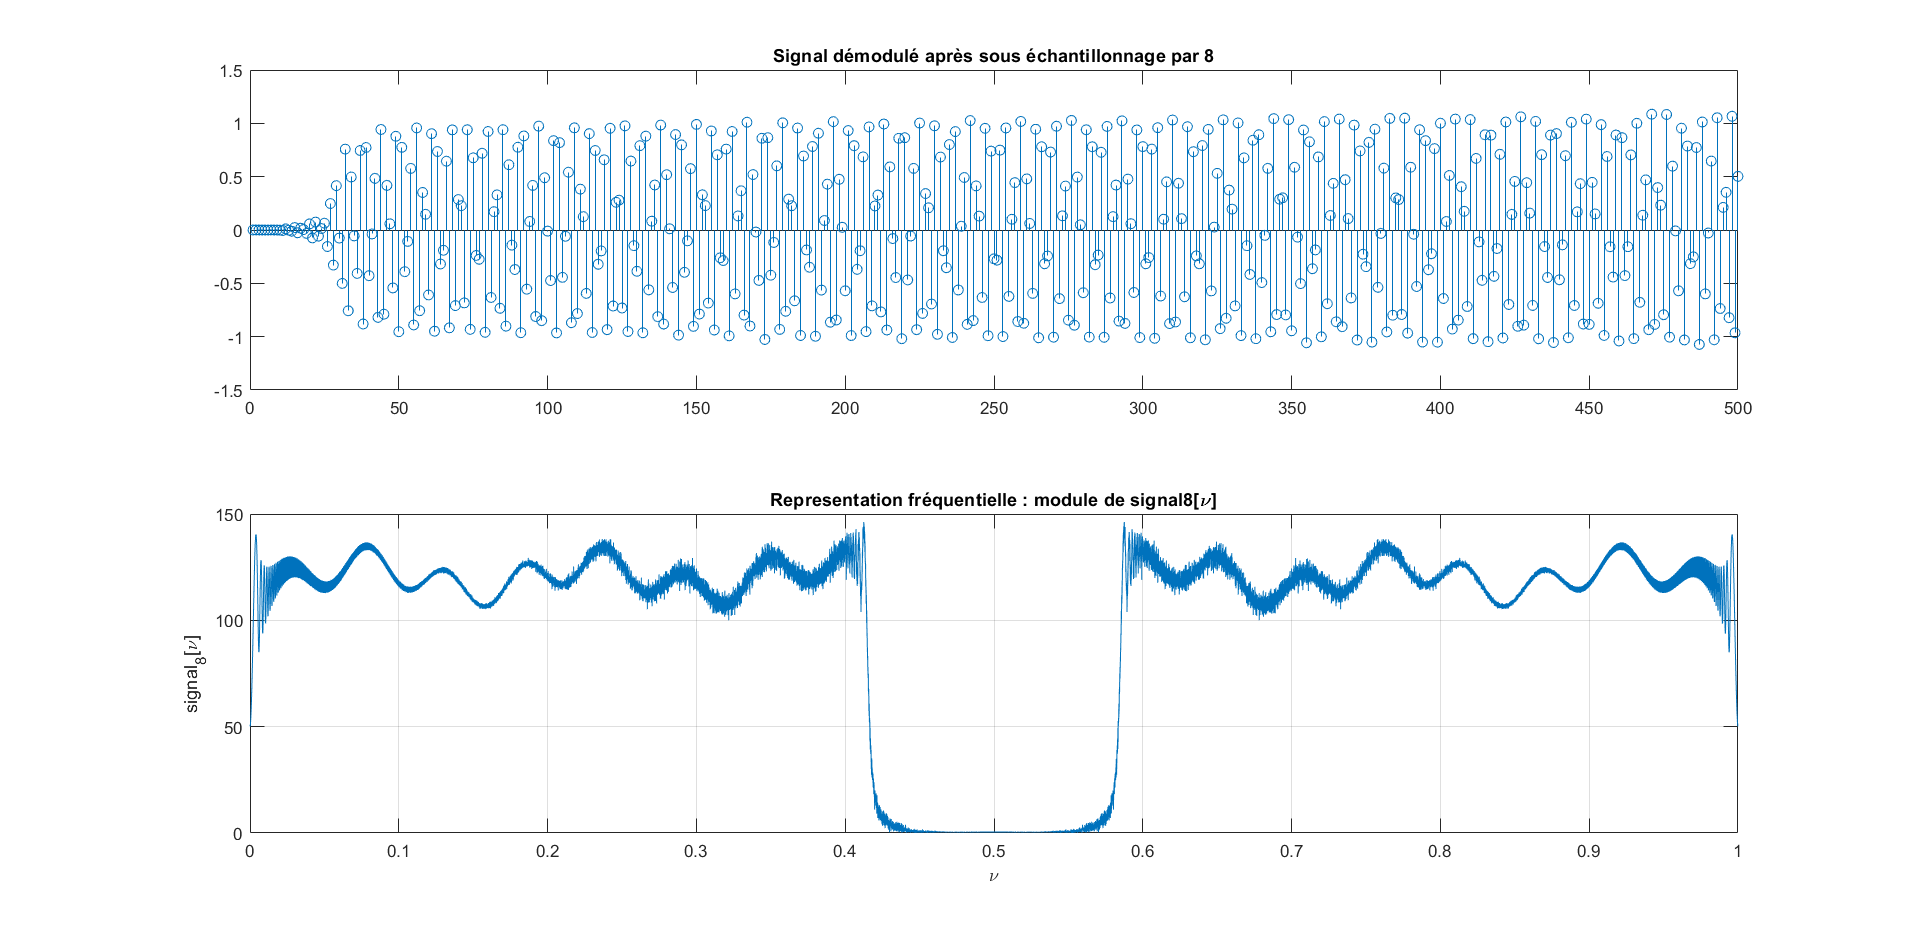
\includegraphics[scale=0.2]{Images/signal8.png}
    \caption{Sortie du sous-échantillonneur par 8}
    \label{fig:sig8}
\end{figure}
\end{frame}

\begin{frame}
\frametitle{Partie 1 : PDM demodulator - PDM modulator} 
\framesubtitle{Démodulateur PDM0 - Améliorations} 
Nous pouvons améliorer le démodulateur PDM en faisant plus d'étapes. En effet, les ordres de nos filtres sont encore assez élevés et créent un certain délai.\\
Nous pouvons faire {8 puis 4 puis 4} ou encore {4 puis 4 puis 4 puis 2}.\\
Plus nous auront de blocs, plus la latence sera minimale.
\end{frame}
%%% FIN PARTIE 1 %%%

%%% PARTIE 2 : SRC %%%
\section{Partie 2 : SRC}
\begin{frame} 
\frametitle{Partie 2 : Sample-Rate Converter} 
\framesubtitle{?} 
?
\end{frame}
%%% FIN PARTIE 2 %%%

\end{document}
